% !TeX spellcheck = en_US
\documentclass[a4paper,fleqn,11pt]{article}

% header
%% Packages

% Styling TOC
\usepackage{tocloft}
\setlength\cftaftertoctitleskip{1cm}
\usepackage[nottoc]{tocbibind}

% Mathe Packages
\usepackage{amsmath,amssymb,epsfig,amsthm,amsfonts,bbm,textcomp}

% Grafiken
\usepackage[font=normalsize,aboveskip=0pt,belowskip=0pt,labelfont=bf]{caption}
\captionsetup{justification=justified,singlelinecheck=false}
\usepackage[edges]{forest}
\usepackage{tikz}
\usetikzlibrary{arrows,intersections,decorations.pathreplacing}
\usepackage[utf8]{inputenc}
\usepackage[T1]{fontenc}
\usepackage{lmodern}
\usepackage[english]{babel}

% Seiten Layout
\usepackage{float}
\usepackage[top=3cm,bottom=3cm,left=3cm,right=3cm,a4paper]{geometry}
\usepackage[onehalfspacing]{setspace}
\usepackage{color}
\usepackage{enumitem}
\usepackage{authblk}

% Fussnoten
\usepackage[flushmargin,hang]{footmisc}
\usepackage{listings}
\usepackage[hyphens]{url}
\usepackage[hidelinks]{hyperref}


% Tabellen
\usepackage{longtable} 			% Lange, mehrseitige Tabelle
\usepackage{tabularx}
\usepackage{array,hhline}
\usepackage{booktabs}			% Linien zwischen Zeilen
\usepackage{multirow}			% Verknüpfte Zellen über Zeilen hinweg
\usepackage{dcolumn}			% Erlaubt variable Orientierung am Decimalpunkt innerhalb einer Zelle
\usepackage{siunitx}

% Wir brauchen auch
\usepackage{todonotes}

% References
\usepackage{natbib}

% Paragraph spacing
\setlength{\parskip}{2ex}

% Spacing around headings
\usepackage[compact]{titlesec}





\begin{document}

% title page

% header

\pagenumbering{Roman}

\title{\huge Forecasting Swiss Exports using Bayesian \\Forecast Reconciliation}

\author[$\dagger$]{Florian Eckert}
\author[$\ddagger$]{Rob J. Hyndman}
\author[$\ddagger$]{Anastasios Panagiotelis}
\affil[$\dagger$]{\small KOF Swiss Economic Institute, ETH Zurich}
\affil[$\ddagger$]{\small Department of Econometrics and Business Statistics, Monash University}
\date{July 2019}

\maketitle
\begin{abstract}
\noindent This paper conducts an extensive forecasting study on 13,118 time series measuring Swiss goods exports, grouped hierarchically by export destination and product category.  We apply existing state of the art methods in forecast reconciliation and introduce a novel Bayesian reconciliation framework. This approach allows for explicit estimation of reconciliation biases, leading to several innovations: Prior judgment can be used to assign weights to specific forecasts and the occurrence of negative reconciled forecasts can be ruled out. Overall we find strong evidence that in addition to producing coherent forecasts, reconciliation also leads to improvements in forecast accuracy.

\noindent \textbf{JEL Classification:} C32, C53, E17\\
\noindent \textbf{Keywords}: Hierarchical Forecasting, Bayesian Forecast Reconciliation, Swiss Exports, Optimal Forecast Combination.
\end{abstract}
\clearpage




% table of contents
%\tableofcontents

%\clearpage

%\listoffigures
%\listoftables

%\clearpage

\pagenumbering{arabic}

			




% 2. Model	
\section{Introduction}
\label{sec:intro}
Forecasting large collections of time series is an important problem in many disciplines, including macroeconomics.  In many cases, time series respect known linear constraints; for instance total exports equal the sum of exports from each trading partner. In such cases, ex post adjustment of forecasts to ensure coherence with these constraints can lead to improvements in forecast accuracy~\citep[see][and references therein]{Wickramasuriya2015}. Despite these successes, existing methodologies for making this adjustment, hereafter referred to as `forecast reconciliation', suffer from some shortcomings.  First, an important theoretical assumption to ensure the optimality of forecast reconciliation is that forecasts are unbiased prior to reconciliation.  Often this assumption will fail to hold in practice.  Second, existing reconciliation methods combine forecasts of different series in a way that is backwards looking - depending on past in-sample forecast errors.  However, in some cases, practitioners may have information that forecasting models may break down even though the have performed well in the past. In this case, some judgmental adjustment of reconciliation methods may be desirable.  The backwards-looking nature of existing reconciliation methods also makes it difficult to exploit information from the entire predictive density of a forecast target.  In this paper we develop new reconciliation techniques using a Bayesian approach that address these shortcomings.

The focus of our empirical study, which represents a significant contribution to the literature in its own right, is Swiss foreign trade in goods. Swiss exports can be disaggregated by destination into geographical regions such as Europe, North America or Australia and then further disaggregated by country. Swiss exports can also be disaggregated into product categories such as precision instruments, textiles or metals and then further disaggregated into subcategories.  Combining these hierarchies leads to a so-called grouped hierarchy \citep{Hyndman2016}. Figure \ref{fig:tree} gives a simple example of grouped structure with $k = 3$ levels, $m = 9$ series in total and $q = 4$ series at the most disaggregate or `bottom' level.
\begin{figure}[H]
	\centering
	\begin{forest}
		before packing={
			forked edges,
		}
		[{$Y_0$}
		[{$Y_{A}$}
		[{$Y_{A1}$}]
		[{$Y_{A2}$}]
		]
		[{$Y_{B}$}
		[{$Y_{B1}$}]
		[{$Y_{B2}$}]
		]
		]
	\end{forest}\hspace{1cm}
	\begin{forest}
		before packing={
			forked edges,
		}
		[{$Y_0$}
		[{$Y_{1}$}
		[{$Y_{A1}$}]
		[{$Y_{B1}$}]
		]
		[{$Y_{2}$}
		[{$Y_{A2}$}]
		[{$Y_{B2}$}]
		]
		]
	\end{forest}
	\vspace{0.4cm}
	\caption[Simple Example of a Grouped Hierarchy]{\textbf{Simple Example of a Grouped Hierarchy.}}
	\label{fig:tree}
\end{figure}
In order to encode the aggregation constraints in a hierarchy, we define $Y_t$ to be an $m$-vector that stacks observations at time $t$ from all series, $Y_{k,t}$ to be a subvector of $Y_t$ containing only the $q$ bottom level series at time $t$ and $S$ to be an $m\times q$  aggregation matrix.  In the simple grouped hierarchy shown in Figure~\ref{fig:tree}, these are given by
\begin{align*}
\underset{(m\times 1)}{Y_t} = \begin{bmatrix}
\ Y_0\ \ \\
\ Y_A\ \ \\
\ Y_B\ \ \\
\ Y_1\ \ \\
\ Y_2\ \ \\
\ Y_{A1}\ \ \\
\ Y_{A2}\ \ \\
\ Y_{B1}\ \ \\
\ Y_{B2}\ \ 
\end{bmatrix} \quad \underset{(m\times q)}{S} &=
\begin{bmatrix}
\ 1 & 1 & 1 & 1 \ \ \\
\ 1 & 1 & 0 & 0 \ \ \\
\ 0 & 0  & 1 & 1\ \ \\
\ 1 & 0 & 1 & 0 \ \ \\
\ 0 & 1 & 0 & 1\ \ \\
\ 1 & 0 & 0 & 0 \ \ \\
\ 0 & 1 & 0 & 0 \ \ \\
\ 0 & 0 & 1 & 0 \ \ \\
\ 0 & 0 & 0 & 1\ \ 
\end{bmatrix} \quad \underset{(q\times 1)}{Y_{k,t}} = \begin{bmatrix}
	\ Y_{A1}\ \ \\
	\ Y_{A2}\ \ \\
	\ Y_{B1}\ \ \\
	\ Y_{B2}\ \ 
\end{bmatrix} 
\end{align*}
Here, and in general, the matrix $S$ is defined so that $Y_t = S Y_{k,t}$ holds for all realized data.  Any vector of forecasts for which the same constraint holds are referred to as `coherent forecasts'. The generality of this setup ensures that forecast reconciliation techniques, including those developed in this paper, work for simpler nested hierarchies as well as for temporal hierarchies~\citep{Athanasopoulos2017}. Earlier literature reduced the issue of producing coherent forecasts as one of selecting a specific level of the hierarchy. For instance the `bottom-up' approach \citep{Gross1990} achieves coherence by producing forecasts for the bottom level series only and then summing these up according to the hierarchical structure. In response to the problem of disagggregated series being noisy and difficult to forecast, a `top-down' approach was proposed \citep[see][and references therein]{Athanasopoulos2009}.  Here, the forecast of the top level series is disaggregated according to the historical or forecast proportions of lower levels. A weakness of the top-down approach is information loss because the time series characteristics at lower levels are not taken into account. A compromise is given by the `middle-out' approach, where the forecasts at an intermediate level of the hierarchy are summed up to get the higher levels and disaggregated to obtain lower level predictions.\\

As an alternative, \cite{Hyndman2011} considered a framework whereby forecasts for all $m$ series and at all levels are produced, referring to these as `base forecasts'.  However, since different, potentially misspecified models are used for individual series, forecasts produced in this fashion are typically incoherent. To reconcile these base forecasts, \cite{Hyndman2011} assumed the following regression structure.
\begin{align}
Y_t(h) &= S\beta_{h} + e_t(h)
\label{eq:regstruct}
\end{align}
where $Y_t(h)$ is an ($m \times 1$) vector containing the h-periods-ahead base forecasts at time $t$ for each level in the hierarchy, $\beta_{h}$ represents the true expected value of the bottom level series and the error term $e_t(h)$ has mean zero and covariance matrix $\Sigma_h$. Reconciled forecasts are given by $Sb_{h}$, where $b_h$ is an estimate of $\beta_{h}$ that combines information about forecasts at all levels. It can be estimated using the following regression equation.
\begin{align}
\label{eq:reg}
b_{h} &= \left(S'W_h^{-1}S \right)^{-1} S'W_h^{-1}Y_t(h)
\end{align}
This choice minimizes the generalized Euclidean distance between $Y_t(h)$ and the reconciled forecasts $Sb_{h}$ with respect to $W_h$. Reconciliation is also guaranteed to reduce the distance to the eventual realization targeted by a forecast. There are several potential choices for $W_h$. Letting $W_h=I$ corresponds to an ordinary least squares estimate.  Alternatively, a high degree of heteroskedasticity in the error terms motivates a diagonal $W_h$ or weighted least squares approach. Under so called `variance scaling', weights are the variances of in-sample $h$-step ahead forecast variances, and forecasts with less accurate historical performance are down-played in reconciliation.  Another alternative is the `nseries' approach due to \cite{Athanasopoulos2017}, whereby weights are based on the number of series aggregated at each node.  More recently, the `MinT' approach was developed by \cite{Wickramasuriya2015} to allow for a $W_h$ that is not diagonal and exploits the covariances between the $h$-step-ahead reconciled forecast errors. The nomenclature MinT refers to the fact that this approach minimizes the trace of the covariance matrix of reconciliation errors.\\

We propose an approach for forecast reconciliation that extends the existing methodology, detailed in section \ref{sec:model}. The main innovation is to convert the structure in equation~\ref{eq:regstruct} into a panel regression. Rather than using a single vector of point forecasts as the dependent variable, we draw samples from the predictive densities of the base forecast models. This panel regression is estimated using Bayesian Markov Chain Monte Carlo algorithms. Our approach has a number of benefits relative to existing methodology. First, reconciliation biases in the base forecasts are made explicit by introducing fixed effects into the panel regression structure. This overcomes a major weakness of existing approaches which require base forecasts to be unbiased to ensure that reconciliation is optimal. Second, we propose a mechanism for down-weighting the influence of particular series irrespective of past forecasting performance. This is valuable if forecasters have strong judgmental reasons for believing that a particular model works particularly well and other base forecasts are less reliable. Third, under our approach, the weights used in reconciliation can depend on the variances of the predictive density rather than in-sample forecast errors.  Existing approaches such as `MinT' and `variance scaling' essentially determine weights based on estimates of the unconditional variance. Our innovation is therefore particularly promising for forecasting models that allow for conditional heteroskedasticity. Fourth, the Bayesian estimation procedure conveniently allows to impose prior information to solve issues such as the occurrence of negative reconciled forecasts. Section \ref{sec:appl} provides a detailed comparison of the method with existing reconciliation techniques using a comprehensive hierarchical dataset of Swiss goods exports. Section~\ref{sec:conc} concludes.

\clearpage

\section{Bayesian Forecast Reconciliation}
\label{sec:model}
\subsection{Model}
As proven extensively in \cite{Timmermann2006}, combining information from different models for the same variable improves the forecast accuracy often substantially. Recent years have seen an increase in the use of model combinations for density forecasts. Besides providing additional information about the uncertainty surrounding a measure of central tendency, density forecasts allow to use this uncertainty for weighting purposes. In the spirit of \cite{Kapetanios2015} or \cite{Cesur2016}, the predictive distributions of the $m$ base forecast models are approximated by drawing samples of size $n$ from the respective distributions. This results in $n$ vectors $\hat{y}_{i}$, each of length $m$, that contain a draw $i$ from each predictive distribution.\footnote{Since every forecast horizon is reconciled independently, the time subscripts are dropped from now on to simplify notation.} The error term consists of two components, a prediction error $e_{i}$ and a reconciliation bias $\alpha$. The latter can be interpreted as a fixed effect that is unique to each forecasted variable. In other terms, $\alpha$ is the difference between the unreconciled forecast mean $\hat{y}$ and the reconciled forecast mean $\tilde{y}$. The interpretation of $\beta$ depends on the definition of $S$, but in general it estimates the mean of the bottom level reconciled forecasts. The following equation can then be used to model the forecast reconciliation.
\begin{align}
\label{eq:main}
\begin{tabular}{ccccccccc}
	$\hat{y}_i$ & $=$ & $\alpha$ & + &$S$ & $\times$ & $\beta$ & $+$ & $e_i$ \\
	$\scriptscriptstyle (m\times 1)$ & & $\scriptscriptstyle (m\times 1)$  & & $ \scriptscriptstyle (m\times q) $ & & $\scriptscriptstyle (q\times 1)$ & & $\scriptscriptstyle (m\times 1)$
\end{tabular}
\end{align}
where $e$ follows a normal distribution with mean zero and covariance matrix $\Sigma$. While $\Sigma$ is not singular by definition because the forecasts in $\hat{y}_{i}$ are not reconciled, it might be near-singular if the base forecasting models are estimated jointly. In the much more common case of independently estimated univariate models, $\Sigma$ is nearly a diagonal matrix. The unreconciled forecasts $\hat{y}_{i}$ follow a multivariate normal distribution.
\begin{align}
\hat{y}\ |\ \alpha,\beta,\Sigma \sim N(\alpha + S\beta,\Sigma)
\end{align}
We are however interested in the reconciled forecasts, which can be obtained by conditioning on $\alpha = 0$. An estimate for the reconciled means is therefore given by the conditional expectation function.
\begin{align*}
\tilde{y} &= \text{E}(S\beta\ |\ \alpha = 0,\Sigma, \hat{y}) = \int \hat{y} f_{\hat{y}|\alpha,\beta,\Sigma}(0,\beta,\Sigma)\ d\hat{y}
\end{align*}
The conditional distributions can be retrieved conveniently from the Gibbs sampling algorithm described in the following subsection. 


\subsection{Estimation}
To account for cross-equation correlations, the reconciliation problem in (\ref{eq:main}) can be expressed as a system of seemingly unrelated regressions. Since the explanatory variables are the same for each equation, it is a special case of the SUR model in \cite{Zellner1962}. However, the parameters are impossible to estimate directly because of perfect multicollinearity in the regressors $I_m$ and $S$. As a result, there is no unique solution available and equation (\ref{eq:main}) represents an ill-posed problem. A convenient answer to this identification issue is given by Bayesian regularization methods. Following \cite{Farebrother1978}, the regression is partitioned in order to separate the parameters that cause multicollinearity.\\

In Bayesian statistics, data is considered to be fixed and parameters are treated as random variables. The researcher has a prior belief about the distribution of the parameters in a model. After observing the data, this prior belief is combined with the likelihood according to Bayes' theorem in order to obtain the posterior distribution of the parameters. This principle can be applied to $\alpha$, $\beta$ and $\Sigma$ in the reconciliation regression.
\begin{align}
	f(\alpha, \beta, \Sigma\ |\ \hat{y}) \propto f(\hat{y}\ |\ \alpha, \beta, \Sigma) \times f(\alpha, \beta, \Sigma)
\end{align}
In other words, the posterior distribution of the bottom-level forecasts is proportional to the likelihood times the prior distribution of the parameters. The likelihood function of the data is then given by
\begin{align*}
f(\hat{y}\ &|\ \alpha,\beta,\Sigma) \propto \frac{1}{|\Sigma|} \exp\left[-\frac{1}{2} \sum_i  (\hat{y}_i - \alpha - S\beta)'\Sigma^{-1}(\hat{y}_i - \alpha - S\beta)\right]
\end{align*}
The joint posterior distribution is accordingly given by
\begin{align*}
f(\alpha,\beta,\Sigma\ |\ \hat{y}) & \propto \frac{1}{|\Sigma|} \exp\left[-\frac{1}{2} \sum_i  (\hat{y}_i - \alpha - S\beta)'\Sigma^{-1}(\hat{y}_i - \alpha - S\beta)\right] \\
&\times \exp \left[-\frac{1}{2}(\alpha - a_0)'A_0^{-1}(\alpha - a_0)\right] \\
&\times \exp \left[-\frac{1}{2}(\beta - b_0)'B_0^{-1}(\beta - b_0)\right] \\
&\times \frac{1}{|\Sigma|(v_0 - m - 1)} \exp \left[-\frac{1}{2} tr(R_0^{-1}\Sigma^{-1}) \right]
\end{align*}
The Bayesian approach has the advantage that uncertainty surrounding the parameters $\alpha$, $\beta$ and $\Sigma$ is taken into account when calculating the conditional expectation of $\tilde{y}$. Following \cite{Percy1992}, we get the marginal distributions by approximating the joint posterior distribution via Gibbs sampling from the conditional distributions.  Convergence is usually achieved very quickly, irrespective of the starting values. It can be verified by testing for stability in the recursive means of the Markov chains. A sufficiently large sample of draws from the joint posterior is saved and evaluated.


\noindent\textbf{Step 1: Draw $\beta$ conditional on $\alpha,\Sigma,\hat{y},S$}\\
The parameter $\beta$ is the mean of the bottom level forecasts, given an appropriate aggregation matrix $S$. The conditional posterior distribution is then given by
\begin{align}
\beta\ |\ \alpha,\Sigma,\hat{y} &\sim N(b_1,B_1)
\end{align}
where
\begin{align*}
B_1 &= \left(\sum_i S'\Sigma^{-1}S + B_0^{-1}\right)^{-1} \\
b_1 &= B_1 \left(\sum_i S'\Sigma^{-1} (\hat{y}_i - \alpha) + B_0^{-1}b_0\right)
\end{align*}
Unless there is reason to believe otherwise, the priors $b_0$ and $B_0$ should be chosen as uninformative as possible. In some cases, this regression approach leads to negative values in the reconciled bottom level forecasts. This might be a concern since many applications such as sales or exports do not allow for negative observations. This issue can be resolved in an uncomplicated fashion during the sampling process by discarding draws of $\beta$ that contain negative entries.\\

\noindent\textbf{Step 2: Draw $\Sigma$ conditional on $\alpha,\beta,\hat{y},S$}\\
$\Sigma$ is the covariance matrix of the prediction errors. It will have a diagonal structure if draws are made from the base predictive distributions independently.  If a joint model is used or if the draws are reordered following \cite{Jeon2018}, $\Sigma$ may have structure on the off-diagonal elements. In the former case, it is fast and simple to draw the variances equation-by-equation from an inverse gamma distribution.  In the latter case $\Sigma$ can be drawn from an inverse Wishart distribution.
\begin{align}
\Sigma\ |\ \alpha,\beta,\hat{y} \sim W^{-1}(v_1,R_1)
\end{align}
where
\begin{align*}
v_1 &= v_0 + n\\
R_1 &=  \left( R_0^{-1} + \sum_i (\hat{y}_i - \alpha - S \beta)'(\hat{y}_i - \alpha - S \beta) \right)^{-1}
\end{align*}
It is useful to set an almost uninformative prior with $v_0$ and $R_0$ very close to zero, which introduces a tiny bit of noise into the reconciled forecasts. This has negligible impact on the posterior distribution, but ensures that $\Sigma$ is nonsingular in the case where a base forecast has no variation. Prediction intervals can also be computed from $\Sigma$, assuming that reconciled and unreconciled forecasts have the same variation.

\clearpage
\noindent\textbf{Step 3: Draw $\alpha$ conditional on $\beta,\Sigma,\hat{y},S$}\\
Because the reconciliation regression is an ill-posed problem, it is necessary to impose additional restrictions on the reconciliation biases $\alpha$ in order to achieve identification. The conditional distribution of $\alpha$ can be expressed equivalently by concentrating out $\beta$ in the following reconciliation identity.
\begin{align}
	\label{eq:prior1}
	\alpha &= \frac{1}{n}\sum_i \hat{y}_i - S\beta
\end{align}
In order to eliminate $\beta$ from equation (\ref{eq:prior1}), both sides are multiplied by a projection matrix $P$. The reconciliation biases depend greatly on the definition of this projection matrix and other choices for $P$ will be discussed in section \ref{sec:weighting}. Using $P = S(S'S)^{-1}S'$ implies an orthogonal projection onto the coherent subspace. The resulting terms are then subtracted from both sides of equation (\ref{eq:prior1}).
\begin{align}
	\label{eq:prior2}
	(I_m - P)\ \alpha &= (I_m - P)\ \frac{1}{n}\sum_i \hat{y}_i  
\end{align}
It is useful to define the idempotent residual maker $M = I_m - P$. Since $M$ is not invertable due to the presence of multicollinearity, equation (\ref{eq:prior2}) cannot be solved for $\alpha$. Multiplying $M$ with $\alpha$ generates the residuals that result from a regression of the reconciliation biases on the aggregation matrix $S$. The generated residuals are by definition the reconciliation biases, which leads to the important identity $M\alpha = \alpha$. This solves the identification problem and leaves the reconciliation biases as a function of the data and the residual maker $M$.\footnote{Should there be the need to compute the Cholesky factor of $M$ for sampling purposes, it can still be inverted by introducing a tiny amount of uncertainty to the diagonal entries. This leads to a negligible bias, but significantly less variation in the parameter estimates. This is referred to as a ridge estimator, developed by \cite{Brown1980} and extended to the seemingly unrelated regression framework by \cite{Haitovsky1987}.} This result is again very intuitive since the reconciliation biases are the residuals from a regression of the base forecasts on the aggregation matrix.
\begin{align}
\alpha &= M\left(\frac{1}{n}\sum_i \hat{y}_i\right)
\end{align}
 Having identified the system in that way, the prior variance $A_0$ is allowed to be uninformative and the prior mean $a_0$ is a zero vector. A numerically stable conditional posterior for $\alpha$ is therefore given by
\begin{align}
	\label{eq:alpha}
	\alpha\ |\ \beta,\Sigma,\hat{y} &\sim N(a_1,A_1)
\end{align}
where
\begin{align*}
	A_1 &= M\Bigg(\frac{\Sigma}{n}\Bigg)M'\\
	a_1 &= M\Bigg(\frac{1}{n}\sum_i \hat{y}_i\Bigg) 
\end{align*}
The precision of this approach can be verified easily by comparing the estimate of $\alpha$ and the reconciliation biases from the fitted values. \\


\subsection{Weighting}
\label{sec:weighting}
The definition of the projection matrix $P$ is crucial for the estimated parameters. Figure \ref{fig:weights} demonstrates the impact of different projections on the estimated reconciliation biases. It features identical unreconciled forecasts of a simple hierarchy with $m=3$ series, where $Y_A + Y_B = Y_0$. For each series a sample is drawn from the predictive forecasts density, assumed to be $N(4,2)$ for $Y_A$ (shown in blue), $N(6,1)$ for $Y_B$ (shown in purple), and $N(16,3)$ for $Y_0$ (shown in yellow). The horizontal axis shows draws from the unreconciled base forecasts, which are clearly incoherent. The vertical axis on the other hand shows the means of the reconciled forecasts. The diagonal line shows values where the means of base and reconciled forecasts are equal.
\begin{figure}[H]
	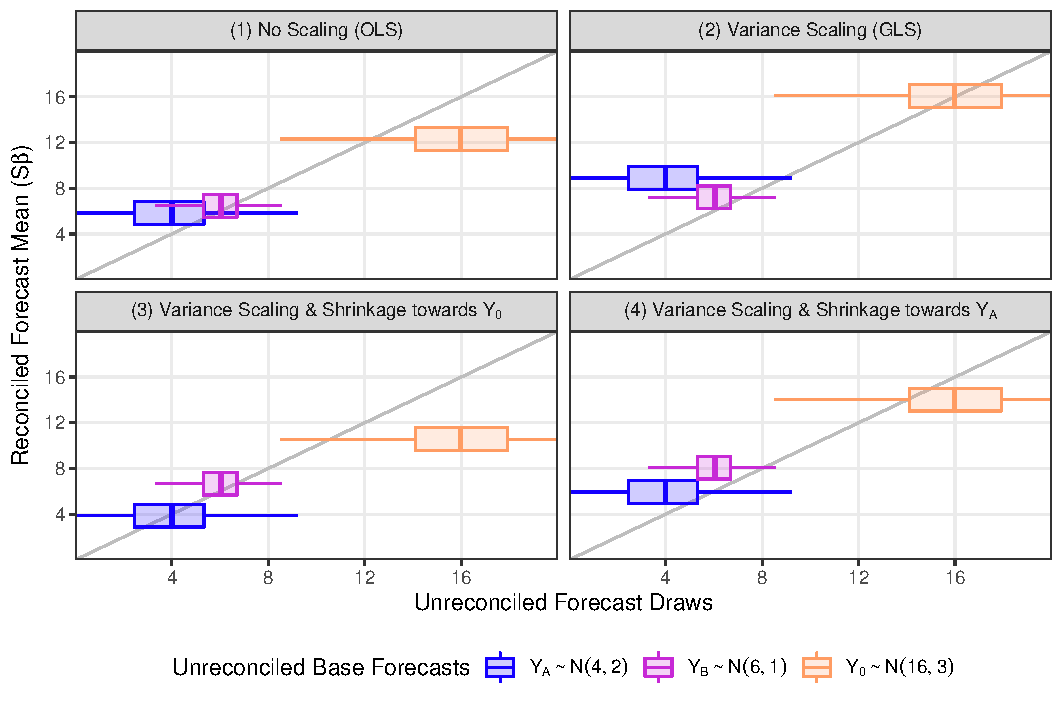
\includegraphics[width=\textwidth]{fig/fig_biases}
	\caption[Weighting Schemes]{\textbf{Weighting Schemes.} \textit{The grey line indicates where the unreconciled base forecasts on the x-axis are equal to reconciled forecast means on the y-axis.}}\label{fig:weights}
\end{figure}
Each panel corresponds to a different choice of $P$. Using $P = S(S'S)^{-1}S'$ corresponds to the orthogonal projection in an ordinary least squares regression. Subfigure (1) shows that the forecast biases for each margin are treated equally, consequently the means of $Y_A$ and $Y_B$ are adjusted upwards while the mean of $Y_0$ is adjusted downwards. Using $P = S(S'\Sigma^{-1}S)^{-1}S'\Sigma^{-1}$ implies that the reconciliation biases are weighted with the inverse of their corresponding forecast variances. This leads to a smaller adjustment in $Y_B$ (the reconciled and base means are close) relative the others since it is more accurate.\\

Even though it is intuitive to weight the reconciliation biases using the predictive accuracy of the corresponding base forecasts, this can be generalized to different weighting schemes. There may exist prior information on the reliability of certain models or the requirement to fix some forecasts at specific values. This could be due to better data availability, higher suitability of a particular model or subjective judgment of the forecaster. This can be achieved by using a projection matrix $P= S(S'(\Lambda\Sigma\Lambda')^{-1}S)^{-1}S'(\Lambda\Sigma\Lambda')^{-1}$ that includes a diagonal matrix of weights $\Lambda$. It might be of interest to selectively shrink some reconciliation biases in $\alpha$ towards zero by decreasing the corresponding entry in $\Lambda$. At the same time, it is necessary to increase the remaining elements such that they are able to capture the higher reconciliation biases at their level of the hierarchy. This is achieved by keeping constant the total dispersion of the  multivariate normal distribution $\Lambda\Sigma\Lambda'$. A common measure is the generalized variance described in \cite{Mustonen1997} and defined as the determinant of a covariance matrix. The weighting matrix $\Lambda$ is therefore always constructed such that the product of the diagonal elements remains constant at 1. This in turn ensures that the total dispersion of $\Lambda\Sigma\Lambda'$ remains equal to the total dispersion of the unweighted $\Sigma$ for all $\Lambda$. Subfigures (3) and (4) shrink the reconciled forecasts of $Y_0$ and $Y_A$ towards their base forecasts.\\

It is important to note that the likelihood is invariant to these choices. Besides the shrinkage of specific reconciliation biases towards zero, there are several other weighting methods conceivable.  Possible approaches include the weighting of each series by its level in the hierarchy or by to the number of series at each node in the hierarchy. This allows for the emulation of the `nseries', `bottom-up', `middle-out' and `top-down' results. A convenient feature of this is that the `middle-out' and `top-down' shrinkage work also for grouped time series, which is not the case in the standard approach. \\

\clearpage


\section{Reconciliation of Export Forecasts}
\label{sec:appl}
\subsection{Data}
We use a comprehensive dataset containing exports of Swiss goods. All time series cover a period from 1988 to 2018 in monthly frequency and are denominated in Swiss francs. They are not adjusted for seasonalities or calendar effects. The data can be grouped by export destination and product category. The geographical hierarchy consists of 8 regions, aggregated from 245 countries and dependent territories. The categorical hierarchy follows a national nomenclature covering 12 main economic groups and 48 subgroups\footnote{Precious metals, precious and semi-precious stones, works of art and antiques are generally omitted in business cycle research due to volatility and structural breaks.}. This leads to a grouped hierarchy with $m = 13'118$ series containing nonzero entries in total and $q = 9'483$ series at the bottom level. Figure \ref{fig:area} shows the historical development of the regional and categorical hierarchies.
\begin{figure}[H]
	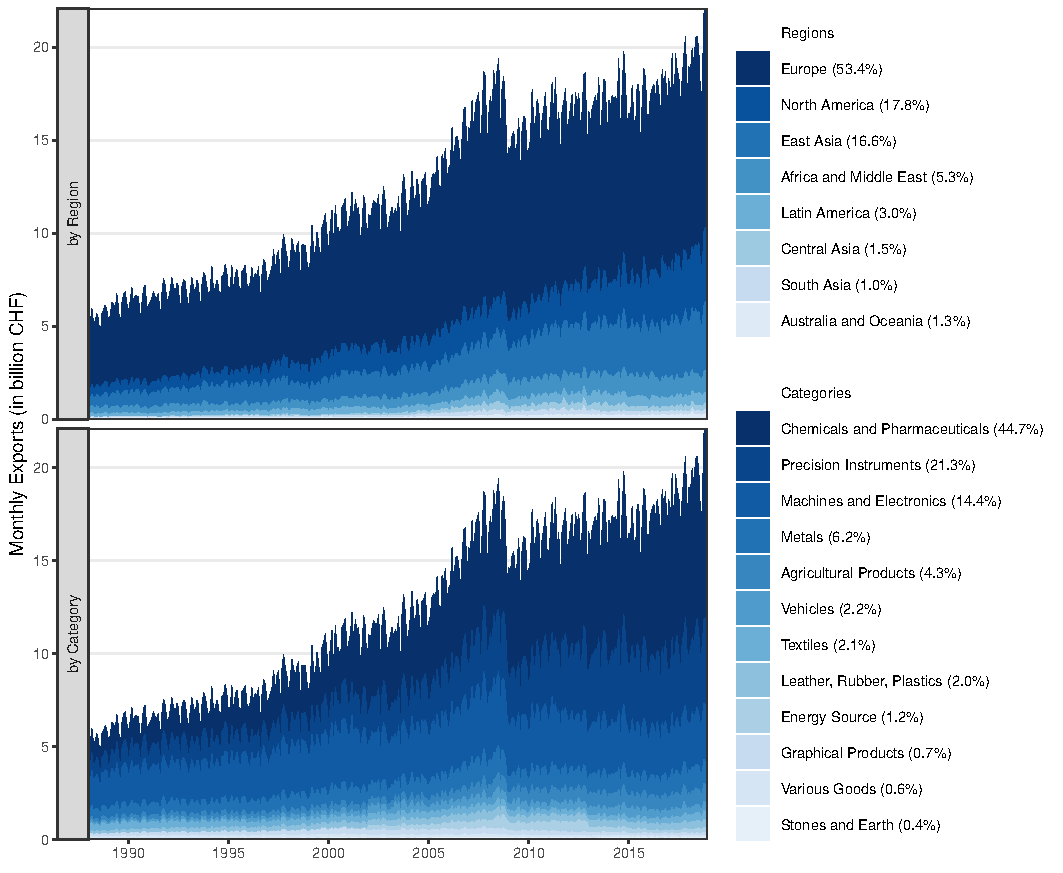
\includegraphics[width=\textwidth]{fig/fig_area}
	\caption[Contribution to Swiss Exports of Goods]{\textbf{Contribution to Swiss Exports of Goods}. \textit{Nominal values, not seasonally adjusted. Average export shares of the year 2018 in parentheses.}}\label{fig:area}
\end{figure}
As a result of its status as a small open economy in a rapidly globalizing world, nominal Swiss exports have increased significantly since the late 1980s. Accounting for more than half of total exports, Europe is a key market for Swiss goods. Increasingly larger shares of exports also go to North America and East Asia with around 17\% each. Exports to Africa and the Middle East, Latin America, Central and South Asia and Australia account only for about 10\% combined.

The hierarchical grouping by categories is more evenly distributed, but has been subject to greater shifts in its composition. The most important categories are `Chemicals and Pharmaceuticals', `Precision Instruments' and `Machines and Electronics'. Figure \ref{fig:treemap} shows the changes in composition between 1988 and 2018.
\begin{figure}[H]
	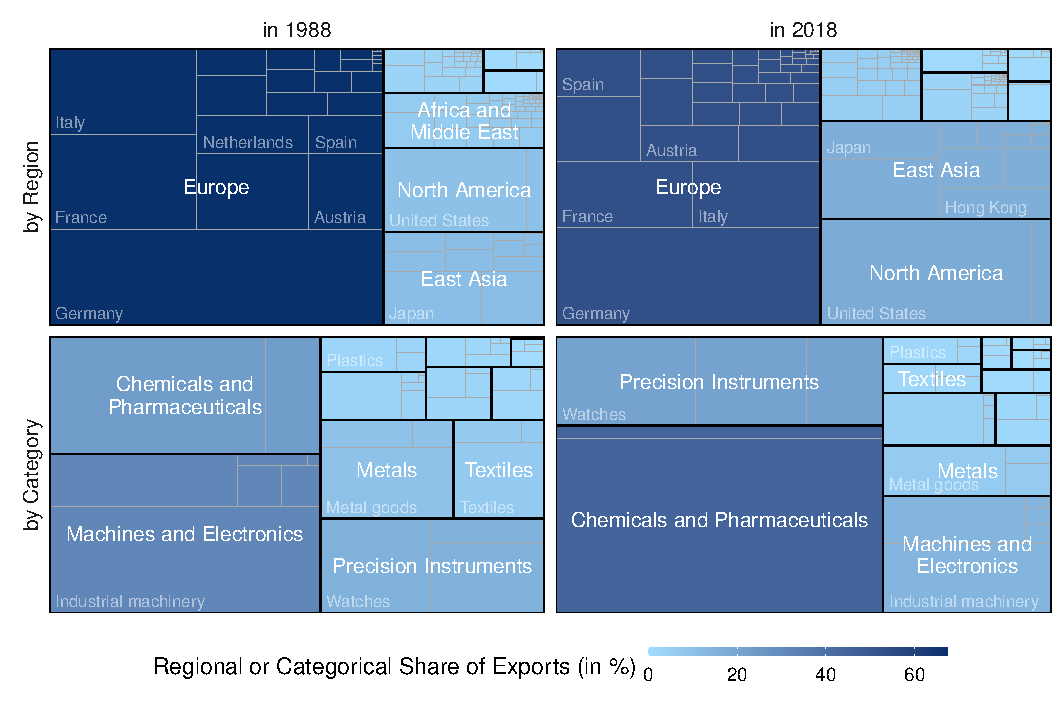
\includegraphics[width=\textwidth]{fig/fig_treemap}
	\caption[Regional and Categorical Composition of Swiss Goods Exports]{\textbf{Regional and Categorical Composition of Swiss Goods Exports.}}\label{fig:treemap}
\end{figure}
The two hierarchical groupings are quite different. The geographic hierarchy with 8 groups and 245 subgroups is very wide. With a majority of the export volume going to European countries, it is nevertheless highly concentrated. This has changed slightly in the past 30 years as the relative share of exports to the rest of the world has increased. The categorical hierarchy on the other hand is rather narrow with 12 groups and 48 subgroups. Compared to the regional hierarchy, the export volume is however more evenly distributed, even though an increasing concentration can be noted.\\

Due to the aggregation involved, top level series are usually less noisy and exhibit more predictable characteristics such as seasonality or trend. Following \cite{Kang2017}, it is possible to construct a measure of predictability for each time series by estimating principal components from a number of time series features that are commonly associated with better predictability. This includes measures such as the strength of seasonality, trend, spectral entropy and serial correlation. Figure \ref{fig:feature} shows the first principal component, which accounts for a large share of the variation in these predictability features.
\begin{figure}[H]
	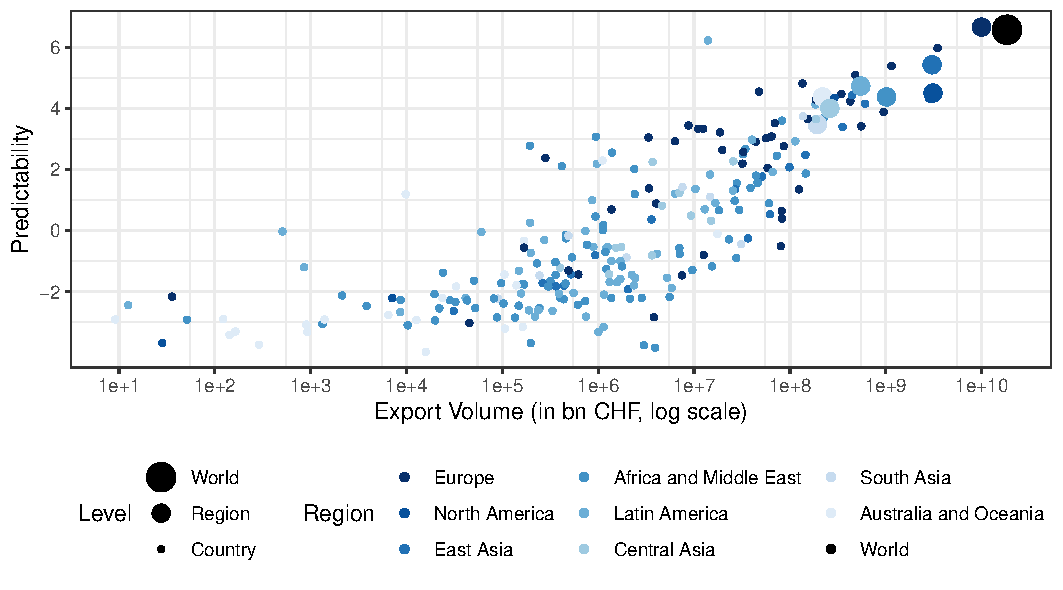
\includegraphics[width=\textwidth]{fig/fig_confetti}
	\caption[Predictability of Different Levels in a Hierarchy]{\textbf{Predictability of Different Levels in a Hierarchy.}\textit{ Predictability is defined as the first principal components of a large number of time series characteristics.}} \label{fig:feature}
\end{figure}
It is evident that there exists a strong correlation between predictability and export volume. This implies that larger series and consequently those at the top of a hierarchy are be easier to forecast. This finding strengthens the claim that reconciliation biases for top level series should be smaller in relative terms than those at the bottom level.\\


\subsection{Setup}
The Bayesian framework and various competing methods are tested by forecasting each month from 1998 to 2018. The expanding training sample starts in 1988 and stops at the end of the year preceding the forecasted month. Various accuracy measures such as the root mean squared error (RMSE), mean absolute percentage error (MAPE) and mean absolute scaled error (MASE) are then calculated over all months of the year following the training sample. The MASE has the advantage of making errors comparable across levels since they are scaled the same. However, the mean squared error is arguably a more appropriate measure for accuracy since it represents the criterion to be minimized in the loss function of the underlying base forecast models. For instance, the mean squared error for the year 2000 is calculated by averaging over the forecasts for all months in the year 2000, using data until December 1999. Gaps between the training and testing samples of one and two years are tested as well in order to check the robustness of the results with different forecasting horizons.\\

For each of the 13'118 series, forecasts are calculated from three models: An autoregressive integrated moving average model (ARIMA), an exponential smoothing state space model (ETS) and a seasonal random walk model (RW). As described in \cite{Hyndman2008}, the model for each series is parametrized automatically based on the Akaike information criterion. In order to get samples from the predictive densities, $n = 1000$ sample paths are simulated from each fitted model. With the exception of the volatile period during the Great Recession, the ARIMA and ETS approaches outperform the Random Walk on average for series at every level and forecasting horizon. All results in the following subsection will therefore rely on ARIMA forecasts using an expanding training sample until the preceding year.\footnote{A comparison of forecasting methods, horizons and accuracy measures can be found in appendix \ref{sec:robust}.}\\

The forecasts are then reconciled using several basic and optimal reconciliation methods. The basic techniques include `bottom-up', `top-down' and `middle-out' reconciliation. The latter two can only be used for non-grouped time series and are therefore tested on the regional and categorical hierarchies separately. The optimal combination methods tested are the ordinary and weighted least squares, nseries, MinT and Bayesian reconciliation approaches. If aggregation of the reconciliation errors is necessary, they are weighted with their respective export share.\\

To test whether the difference between reconciled and unreconciled forecasts is significant at different horizons, the method of \cite{Diebold1995} is used. The Diebold-Mariano test checks for significance in the difference between two squared forecast errors at various forecasting horizons, accounting for serial correlation in the squared error loss. In addition, another significance test is used to compare the mean squared errors directly. Since the prediction errors are assumed to be normally distributed, the ratio between mean squared errors of an unreconciled forecast and a specific reconciled forecast has an $F$-distribution with degrees of freedom corresponding to the number of predictions made. This allows to test for equality of the unreconciled and reconciled mean squared prediction errors.\\


\subsection{Results}
This section provides empirical evidence for the benefits of optimal hierarchical combination. It compares the performance of different reconciliation methods, explores which data characteristics profit in particular from hierarchical combination and provides an example of how selective weighting improves overall forecast accuracy.\\
 
\noindent\textbf{Benefits of Hierarchical Combination.} Figure \ref{fig:rmse} shows the accuracy of forecasts, defined as the mean squared error of the unreconciled forecasts relative to the mean squared errors of the reconciliation methods. Higher bars indicate therefore better forecast performance. The 90\% confidence interval shows the acceptance region of an $F$-test for equality of the mean squared errors. It is worth noting that optimal combination methods and bottom-up forecasts are the only techniques that allows for a consistency across all levels of a grouped hierarchy. Top-down and middle-out reconciliations are not applicable in the case grouped time series.
\begin{figure}[H]
	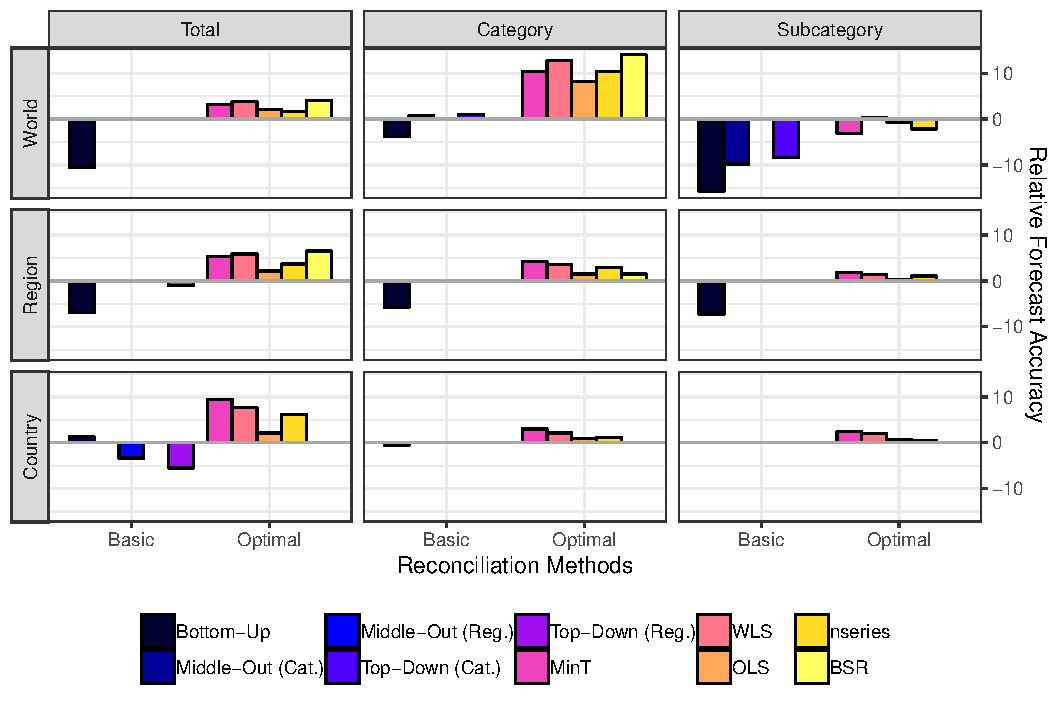
\includegraphics[width=\textwidth]{fig/fig_eval_rmse_relative}
	\caption[Relative Accuracy of Reconciliation Methods]{\textbf{Relative Accuracy of Reconciliation Methods.} \textit{Higher bars indicate better forecasts. Zero line shows the accuracy of unreconciled predictions, with a 90\% confidence interval for the ratio of mean squared errors to be one. Average of all forecast horizons.}} \label{fig:rmse}
\end{figure}

It is evident that the basic reconciliation methods are often not able to beat the unreconciled forecasts and are often significantly worse. The bottom-up reconciliation appears to aggregate a lot of model bias from the lowest levels, whereas the middle-out and top-down approaches fare reasonably well at least for higher levels. Optimal combination forecasts on the other hand tend to outperform the unreconciled forecasts especially for top and middle level series, although not significantly in every instance. The nseries and OLS approaches lead to very volatile results for bottom level series with a low volume, but are still not significantly worse than the unreconciled forecasts. MinT, WLS and BSR estimators work very well for most levels. 

Lower level series appear to benefit less from forecast combination. An exception is the case of misspecified base forecast models. An example is the reclassification of electric energy as a good instead of a service in 2002, which introduced a structural break in the time series. The rigid structure imposed by the hierarchy leads to substantially better forecasts relative to the unreconciled case, especially for the middle level and the weighted least squares approach. Figures \ref{fig:rmseh1}, \ref{fig:rmseh2} and \ref{fig:rmseh3} in the appendix show the relative accuracy at different forecasting horizons. Although the results are very similar, the benefits of hierarchical reconciliation appear to increase when forecasting further into the future.\\

\noindent\textbf{Comparison of Combination Methods.} It is also instructive to look at the development of the relative forecasting accuracy over time in figure \ref{fig:rmse_time}. Even though optimal combination methods are more accurate on average, they do not consistently outperform the unreconciled forecasts. It also appears that MinT, WLS and BSR perform fairly similar over time. For the top level series, the benefits of reconciliation accrued mostly during times of global economic distress and corresponding appreciations of the Swiss franc. The biggest gains can be observed during the early 2000s recession following the burst of the dot-com bubble, the global financial crisis and the following sovereign debt crisis in Europe, and the sudden appreciation of the Swiss franc after the Swiss National Bank stopped supporting the currency peg to the Euro in January 2015.
 \begin{figure}[H]
	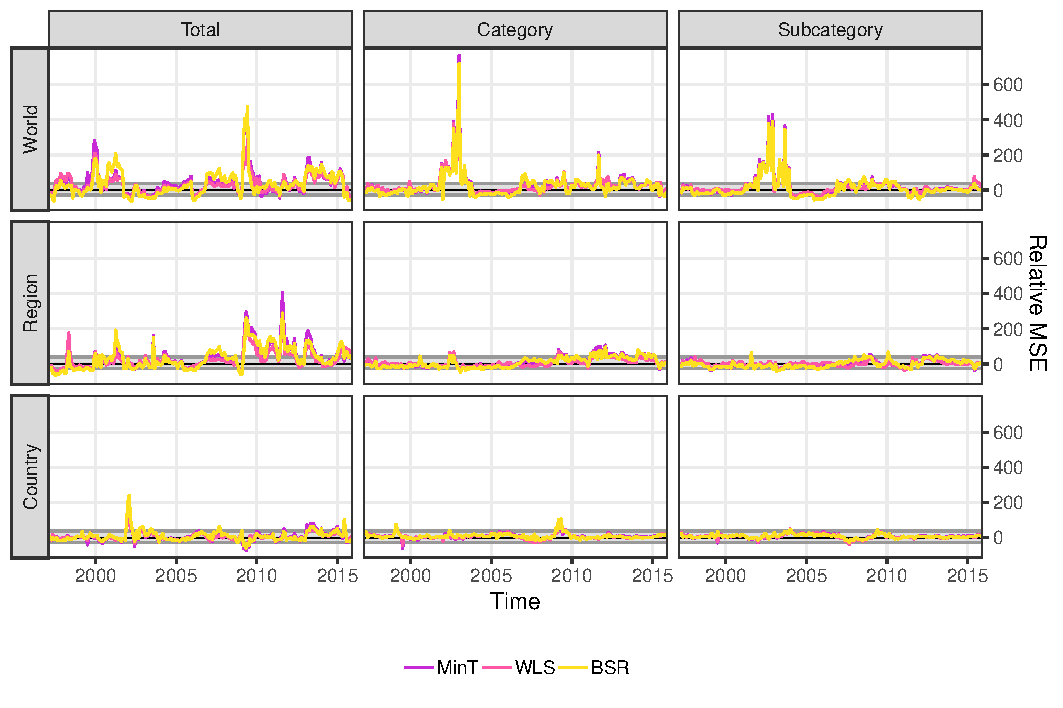
\includegraphics[width=\textwidth]{fig/fig_eval_rmse_time}
	\caption[Relative Accuracy of Reconciliation Methods over Time]{\textbf{Relative Accuracy of Reconciliation Methods over Time.} \textit{Higher lines indicate better forecasts. Zero line shows the accuracy of unreconciled predictions, with a 90\% confidence interval for the ratio of mean squared errors to be one. Base forecasts are generated using ARIMA models. Average of all forecast horizons.}} \label{fig:rmse_time}
\end{figure}


\noindent\textbf{Implications for Data Characteristics.} Another way to dissect the results is to see which time series characteristics increase the benefits from reconciliation. Figure \ref{fig:eval_regions} provides an overview of the relative forecast accuracy by geographical classification, using the Bayesian reconciliation framework. It is again obvious that reconciled forecasts are on average more accurate than in the unreconciled case, but not in every instance. It appears that series with a larger export volume benefit more from reconciliation. Forecasts of exports to Europe, North America and East Asia are almost entirely better off than in the unreconciled case, whereas forecasts of exports to countries with a lower share, such as the islands in Oceania, tend to be worse off. In addition, time series at higher levels in a hierarchy do not necessarily profit more from reconciliation than their corresponding subcategories.
 \begin{figure}[H]
	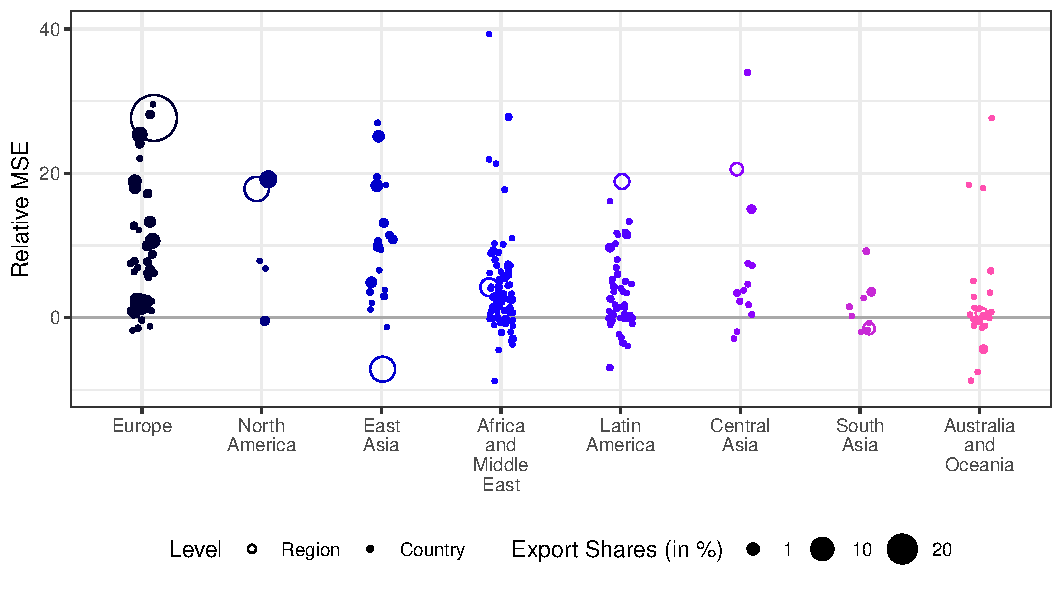
\includegraphics[width=\textwidth]{fig/fig_eval_regions}
	\caption[Relative Accuracy of Reconciliation Methods by Regions]{\textbf{Relative Accuracy of Reconciliation Methods by Regions.} \textit{Higher points indicate better forecasts. Zero line shows the accuracy of unreconciled predictions. Reconciliation using unweighted BSR.}}\label{fig:eval_regions}
\end{figure}
The same results also hold true for the relative forecast accuracy by categories, as shown in figure \ref{fig:eval_categories}. Because the export shares in the categorical hierarchy are more evenly distributed, the pattern of smaller export volumes being worse off due to reconciliation is less pronounced. The category 'energy source`, which exhibits a structural break in the year 2002 with the inclusion of the subcategory 'electrical energy`, is neither on average nor in the year 2002 more accurate than in the unreconciled case. This implies that in the event of misspecified models, the forecast combination improves the accuracy of the remaining hierarchy rather than the misspecified forecast. The results for other optimal combination methods such as weighted least squares and MinT are very similar.

\begin{figure}[H]
	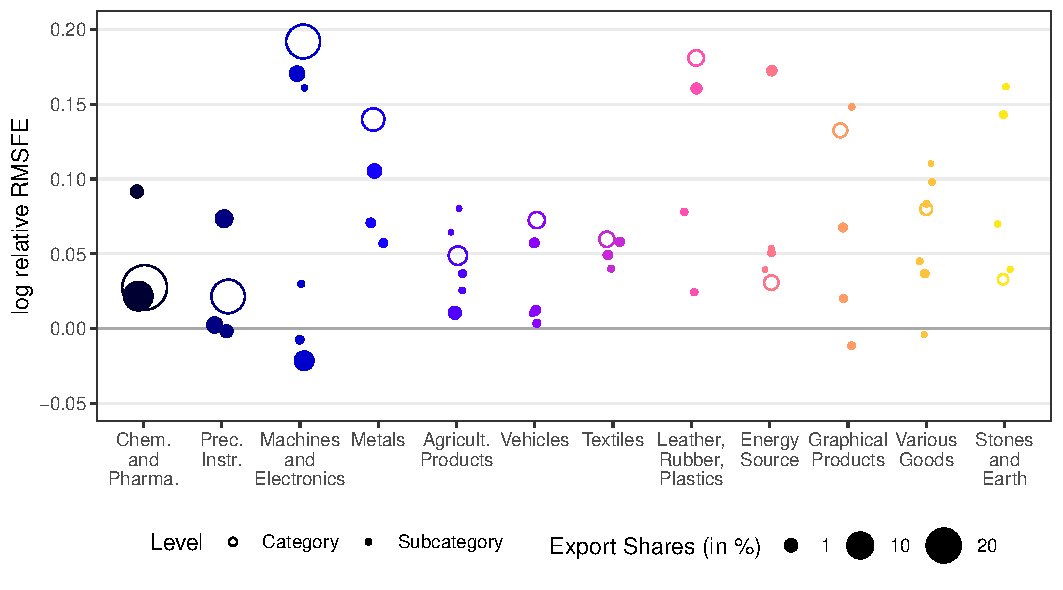
\includegraphics[width=\textwidth]{fig/fig_eval_categories}
	\caption[Relative Accuracy of Reconciliation Methods by Categories]{\textbf{Relative Accuracy of Reconciliation Methods by Categories.} \textit{Higher points indicate better forecasts. Zero line shows the accuracy of unreconciled predictions. Reconciliation using unweighted BSR.}}\label{fig:eval_categories}
\end{figure}

\ \\

\noindent\textbf{Benefits of Selective Shrinkage.} An advantage of the general weighting scheme is that selected series can be shrunk towards their base forecast. This is particularly useful if there exists judgmental information for a particular forecast that would require adjustments for all other base forecasts in a hierarchy. An example is the reclassification of electricity as a good instead of a service. Figure \ref{fig:fcex} shows total exports of energy sources for unweighted and weighted reconciliation.
\begin{figure}[H]
	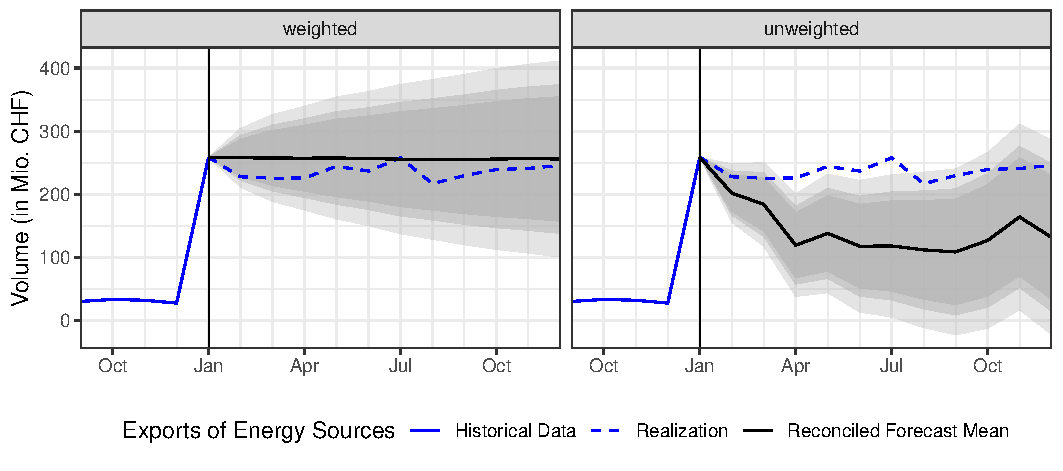
\includegraphics[width=\textwidth]{fig/fig_electricity}
	\caption[Forecast with Bias Weighting]{\textbf{Forecast with Bias Weighting}. \textit{Grey ribbons indicate 90\%, 95\% and 99\% prediction intervals.}}\label{fig:fcex}
\end{figure}
After observing the first value including electric energy in January 2002, a random walk forecast is used for this particular series. Then the series are reconciled with and without an appropriate weighting scheme. For the unweighted model on the right, the other base forecasts assume the structural break to be an outlier and dominate the information from the random walk forecast. Even though the forecaster has prior knowledge that the random walk forecast is accurate, it is overruled in the reconciliation procedure. The only way out would be to adjust the base forecasts for all other series as well, which is very cumbersome.

The model on the left shows the reconciliation of the same forecasts with more weight on the random walk forecast. This is done as described in subsection \ref{sec:weighting}. The diagonal entry in $\Lambda$ that corresponds to the random walk forecast is scaled down. At the same time, the remaining entries are scaled up such that the determinant of $\Lambda$ remains at 1. This forces the reconciled forecast for energy sources to stay close to its random walk base forecast. The remaining series adjust accordingly during the reconciliation procedure. As a result, the mean squared error of the forecast for energy sources in 2002 is more than 90\% lower than in the unweighted case. This also leads to substantial accuracy gains at other levels, while only a few forecast are less accurate. The forecast for total exports for instance is 14\% more accurate.

The prediction intervals are drawn from the conditional posterior distribution of $\Sigma$ and depend therefore on the predictive distributions of the base forecasts. Since the intervals generated by the underlying models tend to be too narrow, the prediction intervals for the reconciled forecasts are too optimistic as well. This issue could be addressed using models more suited for density forecasts or bootstrap aggregation of the exponential smoothing methods \citep{Bergmeir2016}.

\clearpage

\section{Conclusion}\label{sec:conc}
This paper extends the existing literature on hierarchical forecast combination by establishing a Bayesian estimation framework and introducing an explicit definition of the reconciliation biases. This leads to several innovations: It is possible to use prior subjective judgment of the forecaster to shrink reconciled forecasts towards their corresponding base forecasts. The Bayesian sampling procedure allows to impose prior information on the parameters in order to avoid some issues such as the occurrence of negative reconciled forecasts. The use of predictive densities allows for greater flexibility in the choice of the base forecast models. It takes for instance conditional heteroskedasticity into account when weighting the forecasts at different horizons. However, because the approach requires repeated sampling from the joint posterior distribution, it tends to be slower than established reconciliation techniques.

Using a comprehensive dataset of Swiss goods exports, this paper demonstrates that hierarchical combination methods improve the forecasting accuracy significantly compared to the unreconciled case and simpler reconciliation methods. The results are robust to changes in the forecasting horizon, the underlying base forecast models and the measure to determine forecasting accuracy. Optimal combination methods are shown to be particularly useful in the case of misspecified models, during periods of high volatility in the time series and for projections that extend further into the future. Even though the forecasting accuracy is significantly better on average, no reconciliation method consistently outperforms the unreconciled forecasts across series or over time. Forecasts at the top of a hierarchy tend to benefit more from reconciliation than the noisy series at the bottom of a hierarchy. At the same level, series that account for a larger share of the total are on average better of due to reconciliation.

Of the combination methods, the MinT estimator tends to perform slightly better than WLS and BSR. An exception is the case of misspecified base forecast models, where the WLS estimator is more robust. The paper has also provided an example where weighting based on subjective judgment can significantly improve forecast performance. 




\clearpage

% bibliography
\pagenumbering{Roman}
\setcounter{page}{3}
\bibliography{library}
\bibliographystyle{apalike}

\clearpage


% appendix

\appendix
\section{Appendix}


\subsection{Robustness}
\label{sec:robust}

\begin{figure}[H]
	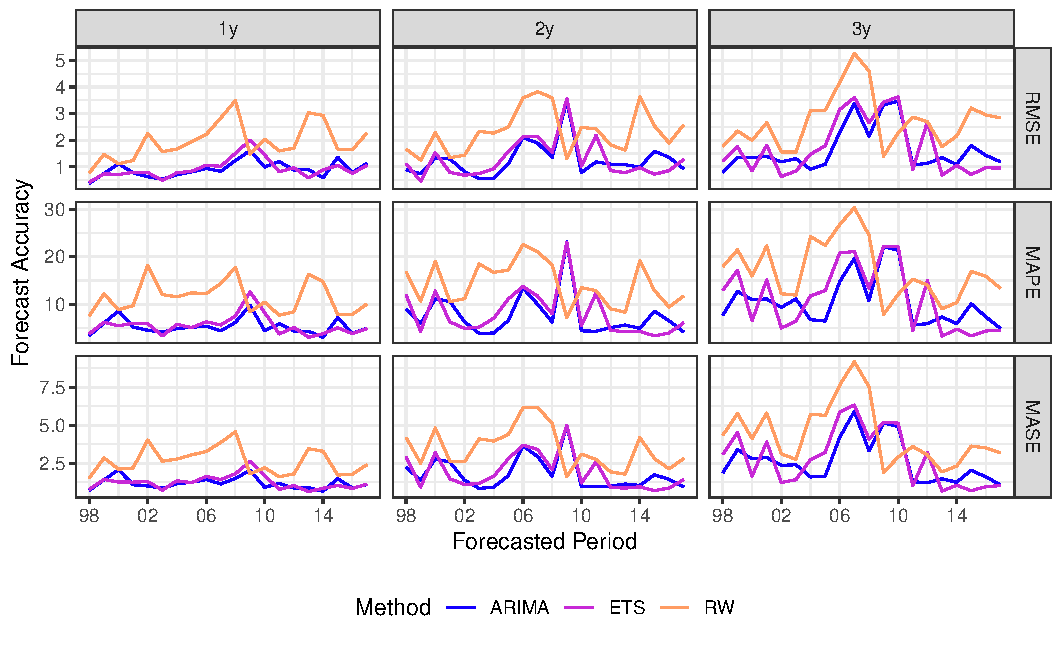
\includegraphics[width=\textwidth]{fig/fig_eval_methods_top}
	\caption{Accuracy of Forecasting Methods at the Top Level}
\end{figure}

\begin{figure}[H]
	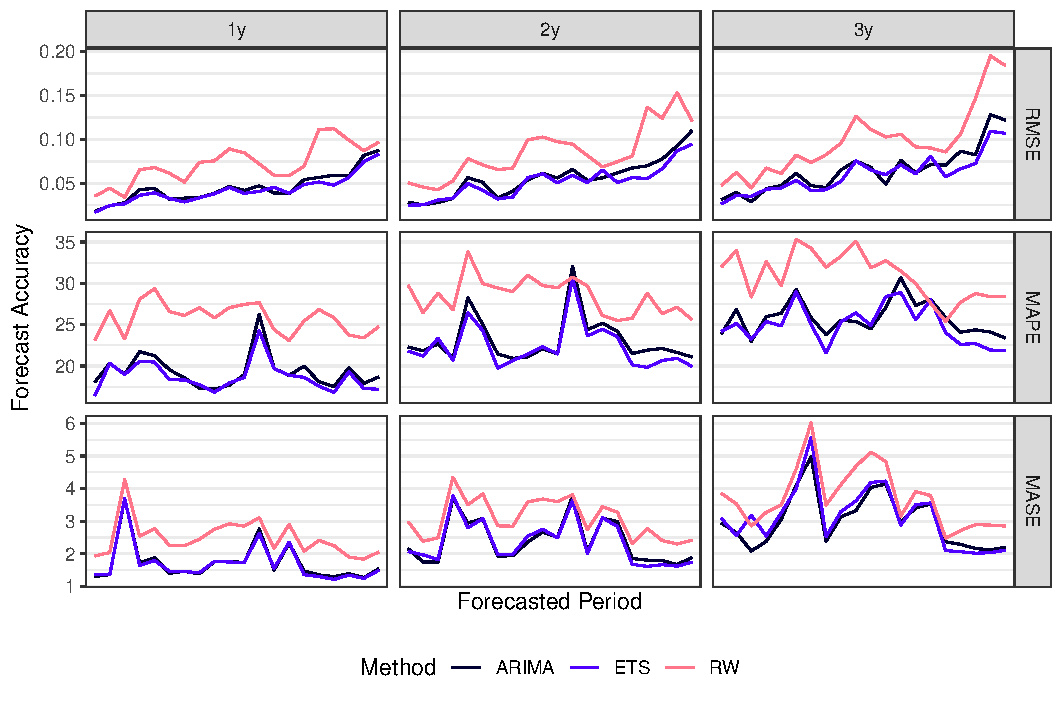
\includegraphics[width=\textwidth]{fig/fig_eval_methods_bottom}
	\caption{Accuracy of Forecasting Methods at the Bottom Level}
\end{figure}


\subsection{Data}
\label{sec:data}
The data is compiled by the Swiss Federal Customs Administration\footnote{\url{https://www.ezv.admin.ch/ezv/en/home/topics/swiss-foreign-trade-statistics.html}} and made available in a machine-friendly format on basis of a subscription.\\
% table with goods categories
\begin{small}
\begin{longtable}{p{2.5cm}p{11.5cm}}
\caption{Tariff Numbers and Descriptions of Goods}\\
\toprule
\normalsize{Tariff Number} & \normalsize{Description}\\
\midrule
\endfirsthead
\multicolumn{2}{@{}l}{\ldots continued}\\
\toprule
\normalsize{Tariff Number} & \normalsize{Description}\\  
\midrule
\endhead
\bottomrule
\multicolumn{2}{r@{}}{continued \ldots}\\
\endfoot
\bottomrule
\endlastfoot
	01	&	Forestry and agricultural products, fisheries	\\
\enskip	01.1	&	Food, beverages and tobacco	\\
\enskip	01.2	&	Feeding stuffs for animals	\\
\enskip	01.3	&	Live animals	\\
\enskip	01.4	&	Horticultural products	\\
\enskip	01.5	&	Forestry products (not firewood)	\\
\enskip	01.6	&	Products for commercial/industrial further processing such as oils, fats, starches, plants and vegetable parts, etc.	\\
\midrule
	02	&	Energy source	\\
\enskip	02.1	&	Solid combustibles	\\
\enskip	02.2	&	Petroleum and distillates	\\
\enskip	02.3	&	Gas	\\
\enskip	02.4	&	Electrical energy	\\
\midrule
	03	&	Textiles, clothing, shoes	\\
\enskip	03.1	&	Textiles	\\
\enskip	03.2	&	Articles of apparel and clothing	\\
\enskip	03.3	&	Shoes, parts and accessories	\\
\midrule
	04	&	Paper, articles of paper and and products of the printing industry	\\
\enskip	04.1	&	Basic materials for paper production, such as cellulose and cellulose fibre and paper and carton waste	\\
\enskip	04.2	&	Paper and carton in rolls, strips or sheets	\\
\enskip	04.3	&	Goods from paper or carton	\\
\enskip	04.4	&	Products of the printing industry	\\
\midrule
	05	&	Leather, rubber, plastics	\\
\enskip	05.1	&	Leather	\\
\enskip	05.2	&	Rubber	\\
\enskip	05.3	&	Plastics	\\
\midrule
	06	&	Products of the chemical and pharmaceutical industry	\\
\enskip	06.1	&	Chemical raw materials, basic materials and unformed plastics	\\
\enskip	06.2	&	Chemical end products, vitamins, diagnostic products, including active substances	\\
\midrule
	07	&	Stones and earth	\\
\enskip	07.1	&	Mineral raw materials and basic products	\\
\enskip	07.2	&	Goods from stone and cement	\\
\enskip	07.3	&	Ceramic wares	\\
\enskip	07.4	&	Glass	\\
\midrule
	08	&	Metals	\\
\enskip	08.1	&	Iron and steel	\\
\enskip	08.2	&	Non-ferrous metals	\\
\enskip	08.3	&	Metal goods	\\
\midrule
	09	&	Machines, appliances, electronics	\\
\enskip	09.1	&	Industrial machinery	\\
\enskip	09.2	&	Agricultural machines	\\
\enskip	09.3	&	Household appliances	\\
\enskip	09.4	&	Office machines	\\
\enskip	09.5	&	Electrical and electronic industry appliances and devices	\\
\enskip	09.6	&	Military equipment	\\
\midrule
	10	&	Vehicles	\\
\enskip	10.1	&	Road vehicles	\\
\enskip	10.2	&	Railed vehicles	\\
\enskip	10.3	&	Air- and spacecraft	\\
\enskip	10.4	&	Watercraft	\\
\midrule
	11	&	Precision instruments, clocks and watches and jewellery	\\
\enskip	11.1	&	Precision instruments and equipment	\\
\enskip	11.2	&	Watches	\\
\enskip	11.3	&	Jewellery and household goods made from precious metals	\\
\midrule
	12	&	Various goods such as music instruments, home furnishings, toys, sports equipment, etc.	\\
\enskip	12.1	&	Exposed film	\\
\enskip	12.2	&	Music instruments	\\
\enskip	12.3	&	Home furnishings	\\
\enskip	12.4	&	Toys and sports equipment	\\
\enskip	12.5	&	Stationery goods	\\
\enskip	12.6	&	Various goods such as umbrellas, neon signs, festive articles, brushes, lighters, pipes, etc.	\\
\midrule
	13	&	Precious metals, precious and semi-precious stones	\\
\enskip	13.1	&	Precious and semi-precious stones	\\
\enskip	13.2	&	Precious metals (including gold and silver bars from 1.1.2012)	\\
\midrule
	14	&	Works of art and antiques	\\
\enskip	14.1	&	Works of art	\\
\enskip	14.2	&	Antiques and collectors' items	\\
\end{longtable}
\end{small}

\clearpage

\begin{small}
	\begin{longtable}{p{7.5cm}cccc}
		\caption{Countries and Regional Aggregates}\\
		\toprule
Country	&	isoCode	&	regCode	&	valid from	&	valid to	\\
		\midrule
		\endfirsthead
		\multicolumn{4}{@{}l}{\ldots continued}\\
		\toprule
Country	&	isoCode	&	regCode	&	valid from	&	valid to	\\
		\midrule
		\endhead
		\bottomrule
		\multicolumn{4}{r@{}}{continued \ldots}\\
		\endfoot
		\bottomrule
		\endlastfoot
Switzerland	&	CH	&	EU	&	01/1988	&	-	\\
Germany	&	DE	&	EU	&	01/1988	&	-	\\
France	&	FR	&	EU	&	01/1988	&	-	\\
Italy	&	IT	&	EU	&	01/1988	&	-	\\
Netherlands	&	NL	&	EU	&	01/1988	&	-	\\
Belgium-Luxembourg	&	BE	&	EU	&	01/1988	&	12/1998	\\
Belgium	&	BE	&	EU	&	01/1999	&	-	\\
Luxembourg	&	LU	&	EU	&	01/1999	&	-	\\
Austria	&	AT	&	EU	&	01/1988	&	-	\\
United Kingdom	&	GB	&	EU	&	01/1988	&	-	\\
Denmark	&	DK	&	EU	&	01/1988	&	-	\\
Norway	&	NO	&	EU	&	01/1988	&	-	\\
Sweden	&	SE	&	EU	&	01/1988	&	-	\\
Portugal	&	PT	&	EU	&	01/1988	&	-	\\
Finland	&	FI	&	EU	&	01/1988	&	-	\\
Croatia, Republic of	&	HR	&	EU	&	02/1992	&	-	\\
Slovenia	&	SI	&	EU	&	02/1992	&	-	\\
Bosnia and Herzegovina	&	BA	&	EU	&	05/1992	&	-	\\
Macedonia	&	MK	&	EU	&	05/1992	&	-	\\
Montenegro	&	ME	&	EU	&	05/1992	&	12/1996	\\
Montenegro	&	ME	&	EU	&	01/2007	&	-	\\
Montenegro	&	XM	&	EU	&	01/2006	&	12/2006	\\
Serbia	&	SQ	&	EU	&	05/1992	&	12/1996	\\
Serbia	&	RS	&	EU	&	01/2007	&	-	\\
Serbia	&	XS	&	EU	&	01/2006	&	12/2006	\\
Federal Republic of Yugoslavia	&	YU	&	EU	&	01/1997	&	12/2003	\\
Serbia and Montenegro	&	CS	&	EU	&	01/2004	&	12/2005	\\
Kosovo	&	XK	&	EU	&	01/2006	&	-	\\
Iceland	&	IS	&	EU	&	01/1988	&	-	\\
Ireland	&	IE	&	EU	&	01/1988	&	-	\\
Spain	&	ES	&	EU	&	01/1988	&	-	\\
Greece	&	GR	&	EU	&	01/1988	&	-	\\
Turkey	&	TR	&	EU	&	01/1988	&	-	\\
GDR	&	DD	&	EU	&	01/1988	&	10/1990	\\
Poland	&	PL	&	EU	&	01/1988	&	-	\\
Czech Republic	&	CZ	&	EU	&	01/1993	&	-	\\
Czechoslovakia	&	CS	&	EU	&	01/1988	&	02/1992	\\
Slovakia	&	SK	&	EU	&	01/1993	&	-	\\
Hungary	&	HU	&	EU	&	01/1988	&	-	\\
Albania	&	AL	&	EU	&	01/1988	&	-	\\
Bulgaria, Republic of	&	BG	&	EU	&	01/1988	&	-	\\
Romania	&	RO	&	EU	&	01/1988	&	-	\\
USSR	&	SU	&	EU	&	01/1988	&	12/1991	\\
Yugoslavia	&	YU	&	EU	&	01/1988	&	04/1992	\\
Cyprus	&	CY	&	EU	&	01/1988	&	-	\\
Svalbard and Jan Mayen Island	&	SJ	&	EU	&	01/1999	&	-	\\
Malta	&	MT	&	EU	&	01/1988	&	-	\\
Gibraltar	&	GI	&	EU	&	01/1988	&	-	\\
Faeroe Islands	&	FO	&	EU	&	01/1988	&	-	\\
San Marino	&	SM	&	EU	&	01/1999	&	-	\\
Holy See	&	VA	&	EU	&	01/1999	&	-	\\
Andorra	&	AD	&	EU	&	01/1988	&	-	\\
Estonia	&	EE	&	EU	&	01/1992	&	-	\\
Latvia	&	LV	&	EU	&	01/1992	&	-	\\
Lithuania	&	LT	&	EU	&	01/1992	&	-	\\
Russian Federation	&	RU	&	CA	&	01/1992	&	-	\\
Armenia	&	AM	&	CA	&	01/1992	&	-	\\
Azerbaijan	&	AZ	&	CA	&	01/1992	&	-	\\
Belarus	&	BY	&	CA	&	01/1992	&	-	\\
Georgia	&	GE	&	CA	&	01/1992	&	-	\\
Kazakhstan	&	KZ	&	CA	&	01/1992	&	-	\\
Kyrgyz, Republic	&	KG	&	CA	&	01/1992	&	-	\\
Moldova, Republic of	&	MD	&	CA	&	01/1992	&	-	\\
Tajikistan	&	TJ	&	CA	&	01/1992	&	-	\\
Turkmenistan	&	TM	&	CA	&	01/1992	&	-	\\
Ukraine	&	UA	&	CA	&	01/1992	&	-	\\
Uzbekistan	&	UZ	&	CA	&	01/1992	&	-	\\
Egypt	&	EG	&	AF	&	01/1988	&	-	\\
Sudan	&	SD	&	AF	&	01/1988	&	-	\\
South Sudan, Republic of	&	SS	&	AF	&	09/2011	&	-	\\
Libya	&	LY	&	AF	&	01/1988	&	-	\\
Tunisia	&	TN	&	AF	&	01/1988	&	-	\\
Algeria	&	DZ	&	AF	&	01/1988	&	-	\\
Canary Islands	&	XA	&	AF	&	01/1988	&	-	\\
Morocco	&	MA	&	AF	&	01/1988	&	-	\\
Western Sahara	&	EH	&	AF	&	01/1999	&	-	\\
Ceuta and Melilla	&	XB	&	AF	&	01/1988	&	12/2010	\\
Equatorial Guinea	&	GQ	&	AF	&	01/1988	&	-	\\
Ceuta	&	XC	&	AF	&	01/2001	&	-	\\
Melilla	&	XL	&	AF	&	01/2001	&	-	\\
Togo	&	TG	&	AF	&	01/1988	&	-	\\
Senegal	&	SN	&	AF	&	01/1988	&	-	\\
Mali	&	ML	&	AF	&	01/1988	&	-	\\
Mauritania	&	MR	&	AF	&	01/1988	&	-	\\
Côte d'Ivoire	&	CI	&	AF	&	01/1988	&	-	\\
Burkina Faso	&	BF	&	AF	&	01/1988	&	-	\\
Benin	&	BJ	&	AF	&	01/1988	&	-	\\
Niger	&	NE	&	AF	&	01/1988	&	-	\\
Guinea	&	GN	&	AF	&	01/1988	&	-	\\
Gambia	&	GM	&	AF	&	01/1988	&	-	\\
Sierra Leone	&	SL	&	AF	&	01/1988	&	-	\\
Liberia	&	LR	&	AF	&	01/1988	&	-	\\
Ghana	&	GH	&	AF	&	01/1988	&	-	\\
Nigeria, Federal Republic of	&	NG	&	AF	&	01/1988	&	-	\\
Cameroon	&	CM	&	AF	&	01/1988	&	-	\\
Gabon	&	GA	&	AF	&	01/1988	&	-	\\
Congo, Republic of the	&	CG	&	AF	&	01/1988	&	-	\\
Central African Republic	&	CF	&	AF	&	01/1988	&	-	\\
Chad	&	TD	&	AF	&	01/1988	&	-	\\
Congo, Democratic Republic of the	&	CD	&	AF	&	06/1997	&	-	\\
Zaire	&	ZR	&	AF	&	01/1988	&	05/1997	\\
Angola	&	AO	&	AF	&	01/1988	&	-	\\
Guinea-Bissau	&	GW	&	AF	&	01/1988	&	-	\\
Botswana	&	BW	&	AF	&	01/1988	&	-	\\
Cabo Verde, Republic of	&	CV	&	AF	&	01/1988	&	-	\\
Lesotho	&	LS	&	AF	&	01/1988	&	-	\\
Sao Tomé and Principe	&	ST	&	AF	&	01/1988	&	-	\\
Namibia	&	NA	&	AF	&	01/1988	&	-	\\
South Africa	&	ZA	&	AF	&	01/1988	&	-	\\
Swaziland	&	SZ	&	AF	&	01/1988	&	-	\\
Zambia	&	ZM	&	AF	&	01/1988	&	-	\\
Zimbabwe	&	ZW	&	AF	&	01/1988	&	-	\\
Malawi	&	MW	&	AF	&	01/1988	&	-	\\
Mozambique	&	MZ	&	AF	&	01/1988	&	-	\\
Madagascar, Republic of	&	MG	&	AF	&	01/1988	&	-	\\
Réunion	&	RE	&	AF	&	01/1988	&	-	\\
St Helena, Ascen. and Tristan da Cunha	&	SH	&	AF	&	01/1988	&	-	\\
Comoros, Union of	&	KM	&	AF	&	01/1988	&	-	\\
Antarctica	&	AQ	&	AF	&	01/1988	&	-	\\
Mauritius	&	MU	&	AF	&	01/1988	&	-	\\
British Indian Ocean Territory	&	IO	&	AF	&	01/1988	&	-	\\
Tanzania, United Republic of	&	TZ	&	AF	&	01/1988	&	-	\\
Seychelles, Republic of	&	SC	&	AF	&	01/1988	&	-	\\
Rwanda	&	RW	&	AF	&	01/1988	&	-	\\
Bouvet Island	&	BV	&	AF	&	01/1999	&	-	\\
Burundi	&	BI	&	AF	&	01/1988	&	-	\\
Mayotte	&	YT	&	AF	&	01/1999	&	-	\\
Somalia, Federal Republic of	&	SO	&	AF	&	01/1988	&	-	\\
French Southern Territories	&	TF	&	AF	&	01/1999	&	-	\\
Djibouti	&	DJ	&	AF	&	01/1988	&	-	\\
Eritrea	&	ER	&	AF	&	01/1994	&	-	\\
Ethiopia, Fed. Democratic Republic of	&	ET	&	AF	&	01/1988	&	-	\\
Kenya	&	KE	&	AF	&	01/1988	&	-	\\
Uganda	&	UG	&	AF	&	01/1988	&	-	\\
Syrian Arab Republic	&	SY	&	AF	&	01/1988	&	-	\\
Lebanon	&	LB	&	AF	&	01/1988	&	-	\\
Israel	&	IL	&	AF	&	01/1988	&	-	\\
Palestine, the State of	&	PS	&	AF	&	01/1997	&	-	\\
Jordan	&	JO	&	AF	&	01/1988	&	-	\\
Saudi Arabia	&	SA	&	AF	&	01/1988	&	-	\\
Yemen (Nord)	&	YE	&	AF	&	01/1988	&	12/1990	\\
Yemen	&	YE	&	AF	&	01/1991	&	-	\\
Yemen (Sud)	&	YD	&	AF	&	01/1988	&	12/1990	\\
Qatar	&	QA	&	AF	&	01/1988	&	-	\\
Bahrain	&	BH	&	AF	&	01/1988	&	-	\\
United Arab Emirates	&	AE	&	AF	&	01/1988	&	-	\\
Oman	&	OM	&	AF	&	01/1988	&	-	\\
Kuwait	&	KW	&	AF	&	01/1988	&	-	\\
Iraq	&	IQ	&	AF	&	01/1988	&	-	\\
Iran, Islamic Republic of	&	IR	&	AF	&	01/1988	&	-	\\
Afghanistan	&	AF	&	SA	&	01/1988	&	-	\\
Pakistan	&	PK	&	SA	&	01/1988	&	-	\\
Bangladesh	&	BD	&	SA	&	01/1988	&	-	\\
India	&	IN	&	SA	&	01/1988	&	-	\\
Sri Lanka	&	LK	&	SA	&	01/1988	&	-	\\
Maldives	&	MV	&	SA	&	01/1988	&	-	\\
Nepal, Federal Democratic Rep.	&	NP	&	SA	&	01/1988	&	-	\\
Bhutan	&	BT	&	SA	&	01/1988	&	-	\\
Myanmar, Union of	&	MM	&	EA	&	01/1988	&	-	\\
Thailand	&	TH	&	EA	&	01/1988	&	-	\\
Malaysia	&	MY	&	EA	&	01/1988	&	-	\\
Brunei Darussalam	&	BN	&	EA	&	01/1988	&	-	\\
Singapore	&	SG	&	EA	&	01/1988	&	-	\\
Cambodia	&	KH	&	EA	&	01/1988	&	-	\\
Lao, People's Democratic Republic	&	LA	&	EA	&	01/1988	&	-	\\
Viet Nam, Socialist Republic of	&	VN	&	EA	&	01/1988	&	-	\\
Mongolia	&	MN	&	EA	&	01/1988	&	-	\\
China, People's Republic of	&	CN	&	EA	&	01/1988	&	-	\\
Hong Kong	&	HK	&	EA	&	01/1988	&	-	\\
Taiwan	&	TW	&	EA	&	01/1988	&	-	\\
Macau	&	MO	&	EA	&	01/1988	&	-	\\
Korea, People's Democratic Republic of	&	KP	&	EA	&	01/1988	&	-	\\
Korea, Republic of	&	KR	&	EA	&	01/1988	&	-	\\
Japan	&	JP	&	EA	&	01/1988	&	-	\\
Philippines	&	PH	&	EA	&	01/1988	&	-	\\
Indonesia	&	ID	&	EA	&	01/1988	&	-	\\
East Timor	&	TL	&	EA	&	01/2004	&	-	\\
East Timor	&	TP	&	EA	&	01/1999	&	12/2003	\\
Canada	&	CA	&	NA	&	01/1988	&	-	\\
St Pierre and Miquelon	&	PM	&	NA	&	01/1988	&	-	\\
United States	&	US	&	NA	&	01/1988	&	-	\\
Greenland	&	GL	&	NA	&	01/1988	&	-	\\
Mexico	&	MX	&	LA	&	01/1988	&	-	\\
Belize	&	BZ	&	LA	&	01/1988	&	-	\\
Guatemala	&	GT	&	LA	&	01/1988	&	-	\\
Honduras	&	HN	&	LA	&	01/1988	&	-	\\
El Salvador	&	SV	&	LA	&	01/1988	&	-	\\
Nicaragua	&	NI	&	LA	&	01/1988	&	-	\\
Costa Rica	&	CR	&	LA	&	01/1988	&	-	\\
Panama	&	PA	&	LA	&	01/1988	&	-	\\
Cayman Islands	&	KY	&	LA	&	01/1988	&	-	\\
Turks and Caicos Islands	&	TC	&	LA	&	01/1988	&	-	\\
Bahamas	&	BS	&	LA	&	01/1988	&	-	\\
Bermuda	&	BM	&	LA	&	01/1988	&	-	\\
Jamaica	&	JM	&	LA	&	01/1988	&	-	\\
Cuba	&	CU	&	LA	&	01/1988	&	-	\\
Haiti	&	HT	&	LA	&	01/1988	&	-	\\
Dominican Republic	&	DO	&	LA	&	01/1988	&	-	\\
American Virgin Islands	&	VI	&	LA	&	01/1988	&	-	\\
Puerto Rico	&	PR	&	LA	&	01/1988	&	12/2005	\\
Dominica	&	DM	&	LA	&	01/1988	&	-	\\
St Vincent and the Grenadines	&	VC	&	LA	&	01/1988	&	-	\\
St Lucia	&	LC	&	LA	&	01/1988	&	-	\\
Montserrat	&	MS	&	LA	&	01/1988	&	-	\\
Antigua and Barbuda	&	AG	&	LA	&	01/1988	&	-	\\
Barbados	&	BB	&	LA	&	01/1988	&	-	\\
Grenada	&	GD	&	LA	&	01/1988	&	-	\\
St Kitts and Nevis	&	KN	&	LA	&	01/1988	&	-	\\
Anguilla	&	AI	&	LA	&	01/1988	&	-	\\
Guadeloupe	&	GP	&	LA	&	01/1988	&	-	\\
British Virgin Islands	&	VG	&	LA	&	01/1999	&	-	\\
Martinique	&	MQ	&	LA	&	01/1988	&	-	\\
Trinidad and Tobago	&	TT	&	LA	&	01/1988	&	-	\\
Saint BarthÈlemy	&	BL	&	LA	&	01/2013	&	-	\\
Netherlands Antilles	&	AN	&	LA	&	01/1988	&	12/2012	\\
Aruba	&	AW	&	LA	&	01/1999	&	-	\\
Bonaire, Sint Eustatius and Saba	&	BQ	&	LA	&	01/2013	&	-	\\
Curacao	&	CW	&	LA	&	01/2013	&	-	\\
Sint Maarten (NL)	&	SX	&	LA	&	01/2013	&	-	\\
Colombia	&	CO	&	LA	&	01/1988	&	-	\\
Venezuela, the Bolivarian Republic of	&	VE	&	LA	&	01/1988	&	-	\\
Guyana	&	GY	&	LA	&	01/1988	&	-	\\
Suriname	&	SR	&	LA	&	01/1988	&	-	\\
French Guiana	&	GF	&	LA	&	01/1988	&	-	\\
Brazil	&	BR	&	LA	&	01/1988	&	-	\\
Paraguay	&	PY	&	LA	&	01/1988	&	-	\\
Uruguay	&	UY	&	LA	&	01/1988	&	-	\\
Argentina	&	AR	&	LA	&	01/1988	&	-	\\
Falkland Islands	&	FK	&	LA	&	01/1988	&	-	\\
South Georgia and South Sandwich Islands	&	GS	&	LA	&	01/1999	&	-	\\
Chile	&	CL	&	LA	&	01/1988	&	-	\\
Bolivia, the Plurinational State of	&	BO	&	LA	&	01/1988	&	-	\\
Peru	&	PE	&	LA	&	01/1988	&	-	\\
Ecuador	&	EC	&	LA	&	01/1988	&	-	\\
Australia	&	AU	&	AO	&	01/1988	&	-	\\
Papua New Guinea	&	PG	&	AO	&	01/1988	&	-	\\
Cocos (Keeling) Islands	&	CC	&	AO	&	01/1999	&	-	\\
Heard and McDonald Islands	&	HM	&	AO	&	01/1999	&	-	\\
Norfolk Island	&	NF	&	AO	&	01/1999	&	-	\\
Christmas Island	&	CX	&	AO	&	01/1999	&	-	\\
New Zealand	&	NZ	&	AO	&	01/1988	&	-	\\
Cook Islands	&	CK	&	AO	&	01/1998	&	-	\\
Samoa	&	WS	&	AO	&	01/1988	&	-	\\
Niue Island	&	NU	&	AO	&	01/1999	&	-	\\
Kiribati, the Republic of	&	KI	&	AO	&	01/1988	&	-	\\
Tokelau Islands	&	TK	&	AO	&	01/1999	&	-	\\
Tuvalu	&	TV	&	AO	&	01/1988	&	-	\\
Pitcairn Islands	&	PN	&	AO	&	01/1988	&	-	\\
Solomon Islands	&	SB	&	AO	&	01/1988	&	-	\\
French Polynesia	&	PF	&	AO	&	01/1988	&	-	\\
New Caledonia	&	NC	&	AO	&	01/1999	&	-	\\
Wallis and Futuna	&	WF	&	AO	&	01/1999	&	-	\\
American Oceania	&	PU	&	AO	&	01/1988	&	12/1996	\\
American Oceania	&	UM	&	AO	&	01/2006	&	-	\\
American Oceania	&	UM	&	AO	&	01/1997	&	12/2005	\\
Northern Mariana, Islands	&	MP	&	AO	&	01/1997	&	-	\\
Marshall Islands	&	MH	&	AO	&	01/1997	&	-	\\
Micronesia, Federated States of	&	FM	&	AO	&	01/1997	&	-	\\
Palau	&	PW	&	AO	&	01/1997	&	-	\\
Fiji, Republic of	&	FJ	&	AO	&	01/1988	&	-	\\
American Samoa	&	AS	&	AO	&	01/2006	&	-	\\
Guam	&	GU	&	AO	&	01/2006	&	-	\\
Vanuatu	&	VU	&	AO	&	01/1988	&	-	\\
Nauru	&	NR	&	AO	&	01/1988	&	-	\\
Tonga	&	TO	&	AO	&	01/1988	&	-	\\
Countries not specified	&	QX	&	EU	&	01/2002	&	-	\\
\end{longtable}
\end{small}

\subsection{Scaling Methods}
\label{subsec:scaling}
by equation (\ref{eq:scale}).
\begin{align}
	\label{eq:scale}
	|\lambda| &= \lambda_1 \lambda_2 \hdots \lambda_m
	= \prod_{s^- = 1}^{x} \lambda_{s^-}\ \eta^{-\frac{1}{x}}   \prod_{s^+ = x+1}^{m} \lambda_{s^+}\ \eta^{\frac{1}{m-x}} = 1
\end{align}
The $x$ local variance components $\lambda_{s^-}$ are scaled down by a factor $\eta^{\frac{1}{x}}$ and the remaining $(m-x)$ components $\lambda_{s^+}$ are correspondingly scaled up by a factor $\eta^{\frac{1}{m-x}}$. The generalized variance remains at unity irrespective of the scaling factor $\eta$ and the number of series to be scaled down $x$. 





\end{document}